\documentclass[a4paper]{article}
\usepackage[utf8]{inputenc}
\usepackage[russian]{babel}
\usepackage[T2A]{fontenc}
\usepackage[warn]{mathtext}
\usepackage{graphicx}
\usepackage{amsmath}
\usepackage{floatflt}
\usepackage[left=20mm, top=20mm, right=20mm, bottom=20mm, footskip=10mm]{geometry}


\graphicspath{ {images/} }
\usepackage{multicol}
\setlength{\columnsep}{2cm}


\begin{document}

\begin{titlepage}
	\centering
	\vspace{5cm}
	{\scshape\LARGE Московский физико-технический институт \par}
	\vspace{4cm}
	{\scshape\Large Лабораторная работа \par}
	\vspace{1cm}
	{\huge\bfseries Петля гистерезиса (статический метод) \par}
	\vspace{1cm}
	\vfill
\begin{flushright}
	{\large группа Б01-303}\par
	\vspace{0.3cm}
	{\LARGE Балдин Виктор}
\end{flushright}


	\vfill

% Bottom of the page
	Долгопрудный, 2024 г.
\end{titlepage}

\section{Цель работы}
Исследование кривых намагничивания ферромагнетиков с помощью баллистического гальванометра

\section{В работе используются:}
\begin{itemize}
    \item генератор тока с блоком питания
    \item тороид
    \item соленоид
    \item баллистический гальванометр с осветителем и шкалой
    \item амперметры
    \item магазин сопротивлений
    \item лабораторный автотрансформатор
    \item разделительный трансформатор
\end{itemize}

\section{Теоретические положения}

\begin{floatingfigure}{41mm}
\noindent
\hfil
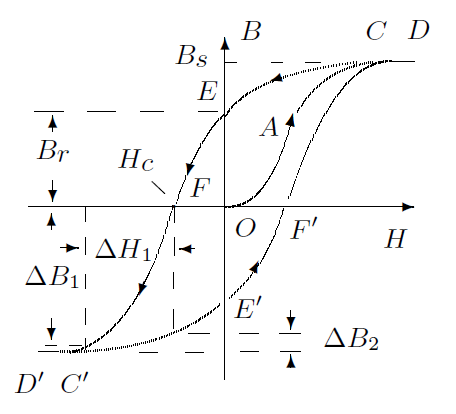
\includegraphics[width=41mm]{fig1.PNG}
\hfil
\caption{Петля гистерезиса ферромагнетика}
\label{figCurvesFF}
\end{floatingfigure}

Магнитная индукция \textbf{B} и напряжённость магнитного поля \textbf{H} в ферромагнетике неоднозначно связаны между собой: индукция зависит не только от напряжённости, но и от предыстории образца. В эксперименте будет исследоваться \textit{основная кривая намагничивания OACD} и \textit{предельная петля гистерезиса DEFD'E'F'D} (см. рис. 1).

С помощью баллистического гальванометра и амперметра будем косвенно измерять зависимость индукции магнитного поля от его напряжённости. \\
Напряжённость магнитного поля \textit{Н} в тороиде зависит от тока, текущего в намагничивающей обмотке:
\begin{equation}
    H = \frac{N_{T_0}}{\pi D}I,
\end{equation}
где $D$ - средний диаметр тора, $N_{T_0}$ - количество витков.

Изменение поля приводит к изменению потока магнитной индукции Ф в сердечнике, в измерительной обмотке возникает ЭДС индукции, через гальванометр, в свою очередь, протекает импульс тока, изменяется положение рамки и, следовательно, зайчика. Окончательно (определив также баллистическую постоянную гальванометра, проведя измерения с соленоидом) для изменения магнитной индукции в сердечнике тороида получаем:
\begin{equation}
    \triangle B = \mu_0 (\frac{d_C}{d_T})^2 \frac{R}{R_1} \frac{N_{C_0}}{N_{T_1}} \frac{N_{C_1}}{l_C} \triangle I_1 \frac{\triangle x}{\triangle x_1},
\end{equation}
где $R$ - полное сопротивление измерительной цепи тороида, $d_C, d_T$ - диаметр поперечного сечения соленоида и тороида соответственно, $N_{C_0}$  - число витков пустотелого соленоида, $N_{C_1}$ - число витков короткой измерительной катушки $l_C$ - длина соленоида, $\triangle x_1$ - отклонение зайчика при работе с соленоидом, $\triangle x$ - отклонение зайчика в эксперименте.

\section{Экспериментальная установка}

\begin{figure}[h]
    \centering
    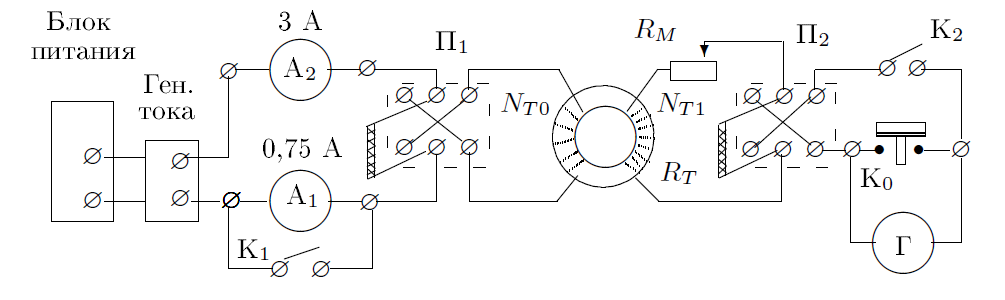
\includegraphics[width=10cm]{fig2.PNG}
    \caption{Схема установки для исследования петли гистерезиса}
    \label{fig:vac}
\end{figure}

% \begin{figure}[h]
%     \centering
%     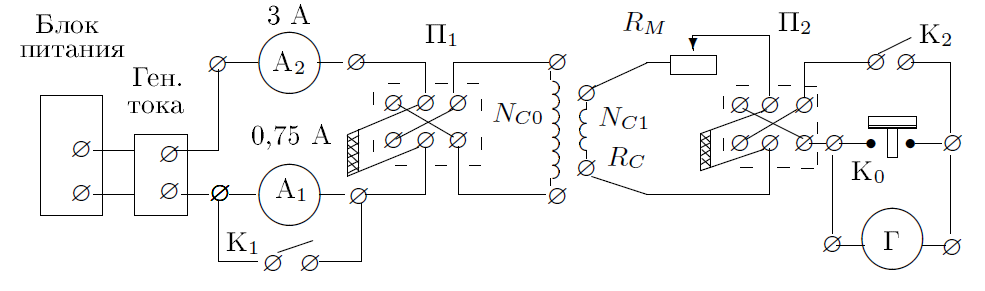
\includegraphics[width=10cm]{fig3.PNG}
%     \caption{Схема установки для калибровки гальванометра}
%     \label{fig:vac}
% \end{figure}

После снятия петли гистерезиса необходимо размагнитить сердечник, подключив его к цепи переменного тока, постепенно снижая его амплитуду. Только затем следует приступать к снятию основной кривой намагничивания.

\section{Ход работы}

\begin{enumerate}
    \item Подготовив к работе экспериментальную установку, снимем зависимость величины скачка $\triangle x$ от величины силы тока в цепи $I$. Пройдём по всей петле гистерезиса, результаты занесём в таблицу 1.

%     \begin{table}[h]
%     \centering
%     \begin{center}
%     \caption{Зависимость $\triangle x$ от $I$ и соответствующие $H$ и $\triangle B$, петля гистерезиса}
%     \end{center}
%     \vspace{0.1cm}
%     \label{tab:my_label}
%     \begin{tabular}{ |p{1.2cm}||p{1cm}|p{1cm}|p{1cm}|p{1cm}|p{1cm}|p{1cm}|p{1cm}|p{1cm}|p{1cm}|p{1cm}|p{1cm}|p{1cm}| }
%  \hline
%     $I$, мA & 538 & 244 & 146.7 & 96.3 & 64.7 & 49.3 & 39.8 & 33.9 & 30.9 & 27.2 & 23.6 & 0.63 \\
% \hline
%     $\triangle x$, см & 6.9 & 6.8 & 4.95 & 3.7 & 2.9 & 1.7 & 1.13 & 0.7 & 0.4 & 0.5 & 0.5 & 4.1 \\
% \hline
%     $H$, А/м & 299.84 & 135.987 & 81.760 & 53.670 & 36.059 & 27.476 & 22.182 & 18.893 & 17.221 & 15.159 & 13.153 & 0.351\\
% \hline
%     $\triangle B$, Тл & 0.002 & 0.211 & 0.166 & 0.124 & 0.097 & 0.057 & 0.038 & 0.023 & 0.014 & 0.010 & 0.007 & 0.007\\
% \hline
% \hline

%     $I$, мА & 0.00 & 0.6 & 23.7 & 27.3 & 31.1 & 34.1 & 40.2 & 49.6 & 64.8 & 96.3 & 146.9 & 244.2 \\
% \hline
%     $\triangle x$, см & 0.1 & 0.1 & 6.9 & 1.6 & 2.3 & 2.45 & 7.5 & 11.8 & 11.3 & 12.2 & 9.3 & 8.9 \\
% \hline
%     $H$, А/м & 0.00 & -0.33 & -13.21 & -15.22 & -17.33 & -19.01 & -22.40 & -27.64 & -36.12 & -53.67 & -81.87 & -136.1 \\
% \hline
%     $\triangle B$, Тл & 0.003 & 0.007 & 0.231 & 0.054 & 0.077 & 0.082 & 0.251 & 0.395 & 0.379 & 0.409 & 0.312 & 0.298 \\

% \hline
% \hline

%     $I$, мА & 537 & 244.1 & 146.8 & 96.3 & 64.8 & 49.3 & 39.8 & 33.9 & 31 & 27.2 & 23.5 & 0.62 \\
% \hline
%     $\triangle x$, см & 17.7 & 11 & 7.85 & 5.8 & 4.6 & 2.6 & 1.8 & 1.15 & 0.6 & 0.8 & 0.8 & 6.4 \\
% \hline
%     $H$, А/м & -299.3 & -136.0 & -81.82 & -53.67 & -36.11 & -27.48 & -22.18 & -18.89 & -17.28 & -15.16 & -13.10 & -0.35\\
% \hline
%     $\triangle B$, Тл & 0.570 & 0.369 & 0.263 & 0.194 & 0.154 & 0.087 & 0.060 & 0.039 & 0.020 & 0.027 & 0.027 & 0.214\\
% \hline
% \hline

%     $I$, мА & 0.00 & 0.6 & 27.3 & 31.1 & 34.1 & 40.1 & 49.6 & 64.9 & 96.4 & 146.8 & 244.1 \\
% \hline
%     $\triangle x$, см & 0.2 & 0.2 & 2.5 & 3.6 & 3.9 & 6.9 & 9.2 & 10.6 & 10.8 & 8.0 & 7.7 & 7.6 \\
% \hline
%     $H$, А/м & 0.000 & 0.351 & 15.215 & 17.333 & 19.005 & 22.349 & 27.643 & 36.170 & 53.726 & 81.815 & 136.043 & 299.841 \\
% \hline
%     $\triangle B$, Тл & 0.007 & 0.005 & 0.084 & 0.121 & 0.131 & 0.231 & 0.308 & 0.355 & 0.362 & 0.268 & 0.258 & 0.255 \\
% \hline
% \hline
%     \end{tabular}
% \end{table}

% \item Отсоединим цепь от тороида, подсоединим её к пустотелому соленоиду. Откалибруем гальванометр. Получившиеся необходимые значения:

% \begin{center}
%     $I_{max}  = 1.473 A$ \hspace{1cm} $\triangle x_{1} = 7.9$ см
% \end{center}

% \item Размагнитим тороид с помощью источника переменного тока и трансформатора. Снимем начальную кривую намагничивания, результаты занесём в таблицу 2.

%    \begin{table}[h]
%     \centering
%     \begin{center}
%     \caption{Зависимость $\triangle x$ от $I$ и соответствующие $H$ и $\triangle B$, начальная кривая намагничивания}
%     \end{center}
%     \vspace{0.1cm}
%     \label{tab:my_label}
%     \begin{tabular}{ |p{1.2cm}||p{1cm}|p{1cm}|p{1cm}|p{1cm}|p{1cm}|p{1cm}|p{1cm}|p{1cm}|p{1cm}|p{1cm}|p{1cm}|p{1cm}| }
%  \hline
%     $I$, мА & 0.6 & 27.3 & 31.1 & 34.1 & 40.1 & 49.6 & 64.9 & 96.4 & 146.8 & 244.1 & 537 \\
% \hline
%     $\triangle x$, см & 0.1 & 5.8 & 1.8 & 2.5 & 2.3 & 5.4 & 8.4 & 11.1 & 15.8 & 15.5 & 18.1 & 18.1 \\
% \hline
%     $H$, А/м & 0.368 & 13.209 & 15.271 & 17.389 & 19.061 & 22.404 & 27.699 & 36.170 & 53.726 & 81.927 & 136.154 & 299.283\\
% \hline
%     $\triangle B$, Тл & 0.001 & 0.100 & 0.031 & 0.043 & 0.039 & 0.093 & 0.144 & 0.191 & 0.266 & 0.271 & 0.294 & 0.311\\
% \hline
% \hline

%     \end{tabular}
% \end{table}

% \item В координатах $B(H)$ построим на одном графике петлю гистерезиса и начальную кривую намагничивания (рисунок 4).

% \begin{figure}[h]
%     \centering
%     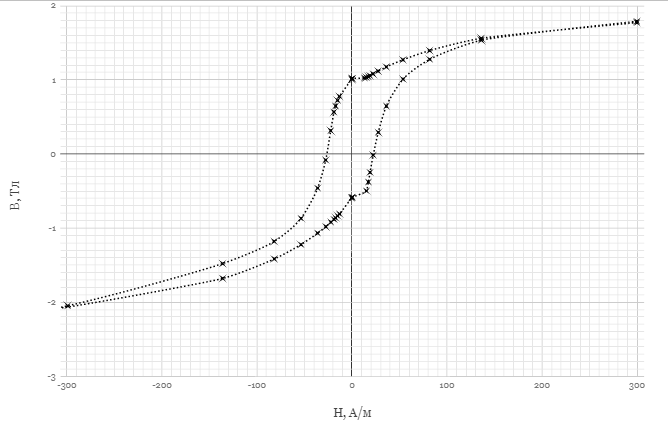
\includegraphics[width=\textwidth]{graph1.PNG}
%     \caption{Петля гистерезиса и начальная кривая намагничивания для исследуемого образца}
%     \label{fig:vac}
% \end{figure}

% По графику определим следующие величины и оценим их погрешности:
% \begin{itemize}
%     \item коэрцитивная сила $H_c$ - значение напряжённости магнитного поля, необходимое для полного размагничивания ферромагнитного вещества равна длине отрезка, высекаемого петлёй гистерезиса на горизонтальной оси. $H_c = 55 \pm 3.3$ А/м.
%     \item индукция насыщения $B_s$ -  максимально достижимое значение внутренней индукции магнитного материала при данной температуре. $B_s = 1.95 \pm 0.3$ Тл.
%     \item максимальная дифференциальная магнитная проницаемость $\mu_d = \frac{1}{\mu_0}\frac{dB}{dH}$ - характеризующий связь между магнитной индукцией B и напряжённостью магнитного поля H в веществе. $\mu_d = 9715 \pm 270$
% \end{itemize}

% Итоговые результаты сведём в таблицу. Теоретические значения возьмём из справочника в пособии к лабораторным работам для технической стали.

%    \begin{table}[h]
%     \centering
%     \begin{center}
%     \caption{Соответствие теоретических и экспериментальных результатов}
%     \end{center}
%     \vspace{0.1cm}
%     \label{tab:my_label}
%     \begin{tabular}{ |p{2cm}||p{3cm}|p{3cm}| }
%  \hline
%      & Эксперимент & Справочник\\
% \hline
% \hline
%      $H_c$, А/м & $55 \pm 3.3$ & 80  \\
% \hline
%     $B_s$, Тл & $1.95 \pm 0.3$ & 2.15 \\
% \hline
%     $\mu_0$ & $9715 \pm 270$ & 5000 \\
% \hline

%     \end{tabular}
% \end{table}

% \section{Вывод}

% В ходе работы были исследованы петля гистерезиса магнитомягкого материала, его начальная кривая намагничивания, с хорошей точностью экспериментально определены некоторые магнитные свойства. По кривой гистерезиса видно, что материал является магнитомягким, так как площадь петли мала. Также она симметрична и в целом соответствует теоретическим изображениям подобных кривых. Различие справочных и экспериментальных данных может объясняться тем, что, скорее всего, образец изготовлен не из чисто технического железа, а из сплава его с другим металлом.

\end{enumerate}

\end{document}
